\begin{figure}[!htb]
\begin{center}
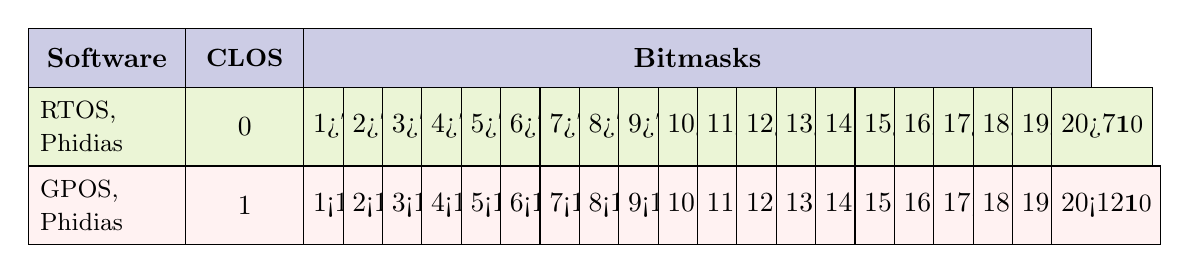
\begin{tikzpicture}

	\node at (0.5,2)[rectangle, draw=black, fill=NavyBlue!20, minimum height = 0.75cm, minimum width = 10cm, anchor=south west] (bitmasks) {\textbf{Bitmasks}};
	\node at (-1.0,2)[rectangle, draw=black, fill=NavyBlue!20, minimum height = 0.75cm, minimum width = 1.5cm, anchor=south west] (clos) {\textbf{\small{CLOS}}};
	\node at (-3.0,2)[rectangle, draw=black, fill=NavyBlue!20, minimum height = 0.75cm, minimum width = 2cm, anchor=south west] (soft) {\textbf{Software}};

	\node at (-1.0,1)[rectangle, draw=black, fill=YellowGreen!20, minimum height = 1cm, minimum width = 1.5cm, anchor=south west] (clos0) {0};
	\node at (-1.0,0)[rectangle, draw=black, fill=pink!20, minimum height = 1cm, minimum width = 1.5cm, anchor=south west] (clos1) {1};
	\node at (-3.0,1)[rectangle, draw=black, fill=YellowGreen!20, minimum height = 1cm, minimum width = 2cm, anchor=south west, text width=1.7cm]
				 (soft0) {\small{RTOS, Phidias}};
	\node at (-3.0,0)[rectangle, draw=black, fill=pink!20, minimum height = 1cm, minimum width = 2cm, anchor=south west, text width=1.7cm] 
				(soft1) {\small{GPOS, Phidias}};

	\foreach \x in {1,...,20}
		    	\node at (0.5*\x,1)[rectangle, draw=black, fill=YellowGreen!20, minimum height = 1cm, minimum width = 0.5cm, anchor=south west] (c1\x) 
							{\ifthenelse{\x>7}{\small{\textbf{1}}}{\small{0}}};

	\foreach \x in {1,...,20}
		    	\node at (0.5*\x,0)[rectangle, draw=black, fill=pink!20, minimum height = 1cm, minimum width = 0.5cm, anchor=south west] (c2\x) 
							{\ifthenelse{\x<12}{\small{\textbf{1}}}{\small{0}}};


\end{tikzpicture}
\end{center}
\ifreport
\caption{LLC Partitioning in Virtual Setup}
\fi
\label{fig-vsetup-cat-bitmasks}
\end{figure}
